\section{Cantor's Theorem,...again}
Now that we have been thinking about Cantor's theorem, infinities, and functions for a while, let's have another fresh look at the proof of Cantor's theorem.  This time we will be armed with tools and skills to discuss it like mathematicians!

\begin{quotation}
\noindent Suppose there is a planet where infinitely many people live. They form every possible group. Every group is uniquely named after a person who is not in that group. Now take the group where there are all the people who have groups named after them. What's the name of it then?\\

\hfill YouTube - Zsigmond Telek  1 year ago
\end{quotation}

I think there two proofs I woud like to explore that prove Cantor's theorem: one used a contradiction (or paradox) and the other uses a construction.  Both of these proof techniques are worth exploring due to the fact that they are employed often in mathematics.  So here we go:

\begin{theorem}[Cantor's Theorem]
The cardinality of a power set is greater than the cardinality of that set.
\end{theorem}

The theorem statement is simple.  But the proof is perhaps less so.

\begin{proof}
For two sets to have the same cardinality, there must be a bijection between them.  
\begin{figure}[ht]
\centering
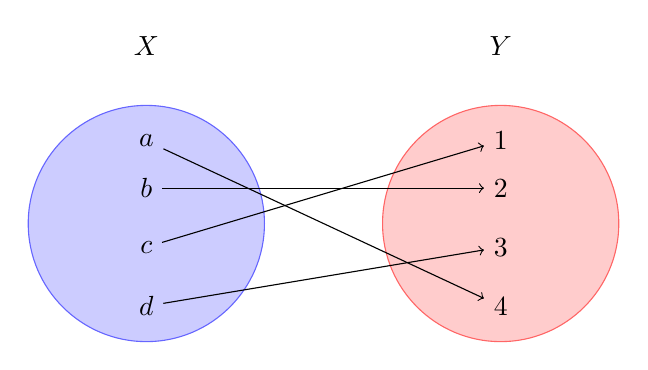
\begin{tikzpicture}[scale=1.50]
    % draw the sets
    \filldraw[fill=blue!20, draw=blue!60] (-1.5,0) circle (1cm);
    \filldraw[fill=red!20, draw=red!60] (1.5,0) circle (1cm);
    % the texts
    \node at (-1.5,1.5) {$X$};
    \node at (1.5,1.5) {$Y$};
    % the points in the sets (here I just create nodes to use them later on to position
    % the circles and the arrows
    \node (x1) at (-1.5,0.7) {$a$};
    \node (x2) at (-1.5,0.3) {$b$};
    \node (x3) at (-1.5,-0.2) {$c$};
    \node (x4) at (-1.5,-0.7) {$d$};
    \node (y1) at (1.5,0.7) {$1$};
    \node (y2) at (1.5,0.3) {$2$};
    \node (y3) at (1.5,-0.2) {$3$};
    \node (y4) at (1.5,-0.7) {$4$};
%    % draw the arrows
    \draw[->] (x1) -- (y4);
    \draw[->] (x2) -- (y2);
    \draw[->] (x3) -- (y1);
    \draw[->] (x4) -- (y3);
\end{tikzpicture}
\caption{A simple example of a bijection between $X$ and $Y$.}
\end{figure}
A bijection is both injective and surjective (verify this for yourself).  The spirit of this proof is to show that, although there exists injections from a set to its power set, there does not exist a surjection, and therefore there can not be a bijection.

%\begin{enumerate}
%\item
 First we show that there exists an injection.  To prove that something exists, we need only find an example of it.  To prove that forest gnomes exist, we only need to find an example of a forest gnome, then everyone would have to finally agree that forest gnomes are real, they have rights, and deserve equal representation.  It is as simple as that!

Similarly, to show that  injections between a set and its power set exist, we only need to find an example of one.  I am providing an example here in Example \ref{injection01}

%Let $f: X\mapsto Y$ such that for $x\in X, ~~f(x)  = \{x\}$.  

\begin{example}[$f: X\mapsto Y$ such that for $x\in X, ~~f(x)  = \{x\}$.]
Consdier the infinite set of the natural numbers, $N = \{1,2,3,\cdots\}$.  Now $f(x)$ is simply the set containing $x$, i.e. $\{x \}$.  So $f(3) = \{3\}, ~f(4) = \{4\}$ and so on.  
\begin{proof}Let's prove that this is injective.

\notes{10}
\end{proof}
Now we know that there exists both forest gnomes and injections between a set (even and infinite set) and its power set. \label{injection01}
\end{example}

...Back to the proof of Cantor's theorem.
\begin{remark} An important and relevant observation is that in this previous example, $f(x)	\subseteq \powerset (N)$.  Explain why this is true.
\notes{5}


\ifKey\hfill\begin{minipage}{0.5\textwidth}\color{red}
The power set is simply the set of all sets.  So if the function maps $x$ onto a set $\{x \}$, then that must be in the power set.  We will use this idea again shortly.
\color{black}\end{minipage}
\fi
\end{remark}

\begin{problem} [$\left| \powerset (N) \right| \ge \left | N\right|$]
Having shown that there exists an injection between $N$ and $\powerset (N)$ implies the cardinality of the power set of $N$ is greater than the cardinality of $N$, i.e. $\left| \powerset (N) \right| \ge \left | N\right|$.  Why?
\notes{10}

\ifKey\hfill\begin{minipage}{0.5\textwidth}\color{red}$\forall x\in N, \exists f(x)\in\powerset$, so there has to be at least that many members.
\color{black}\end{minipage}
\fi 
\end{problem}

%\item 
So at this point we have established that $\left| \powerset (N) \right| \ge \left | N\right|$.  To prove that these cardinalities are strictly unequal we need to remove the possibility that $\left| \powerset (N) \right| = \left | N\right|$.  This can be done by showing that, in fact, no surjection exists between $N$ and $\powerset (N)$.  If we can do this, then we have shown that no bijection can exist, meaning no one to one correspondance, and we are done.  
%\end{enumerate}

%\item 

Suppose, to the contrary, that we have a surjection (we will soon show this is impossible).  Let this be $g(x)$.  Recall what a surjection is!
$$ \forall y\in \powerset (N), \exists~ x\in N \textrm{ such that } g(x) = y$$
\begin{figure}[h]
\centering
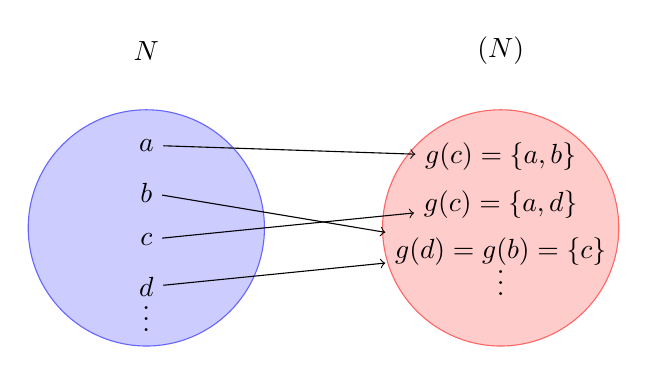
\begin{tikzpicture}[scale=1.50]
    % draw the sets
    \filldraw[fill=blue!20, draw=blue!60] (-1.5,0) circle (1cm);
    \filldraw[fill=red!20, draw=red!60] (1.5,0) circle (1cm);
    % the texts
    \node at (-1.5,1.5) {$N$};
    \node at (1.5,1.5) {$\powerset (N)$};
    % the points in the sets (here I just create nodes to use them later on to position
    % the circles and the arrows
    \node (x1) at (-1.5,0.7) {$a$};
    \node (x2) at (-1.5,0.3) {$b$};
    \node (x3) at (-1.5,-0.1) {$c$};
    \node (x4) at (-1.5,-0.5) {$d$};
    \node (x5) at (-1.5,-0.7) {$\vdots$};
        
    \node (y1) at (1.5,0.6) {$g(c) = \{a, b \}$};
    \node (y2) at (1.5,0.2) {$g(c) = \{a, d \}$};
    \node (y3) at (1.5,-0.2) {$g(d) = g(b) = \{c \}$};
    \node (y4) at (1.5,-0.4) {$\vdots$};
%    % draw the arrows
    \draw[->] (x1) -- (y1);
    \draw[->] (x2) -- (y3);
    \draw[->] (x3) -- (y2);
    \draw[->] (x4) -- (y3);
\end{tikzpicture}
\caption{A simple example of a surjection between $X$ and $Y$.  Every $Y$ has at least one $X$}
\end{figure}
In other words, , whatever $x$ from $N$ we choose, the \emph{image} of $x$, i.e. $g(x)$, is in the power set, $\powerset (N)$.

But what does it mean to be ``in the power set"?
\notes{5}

\ifKey
\hfill\begin{minipage}{0.5\textwidth}\color{red} $g(x)\subset N$ because $\powerset (N)$ is the set of all subsets of $N$.
\color{black}\end{minipage}
\fi

In other words,
$$\forall x \in N, g(x)\subseteq N $$ 

This is what we must show does \textbf{not} exist, or is impossible, or is a forest gnome.  We accomplish this by finding a subset of $N$ that is not in the image of $g$.  

\subsection*{We will use Cantor's special set, his diagonal set, $\mathcal{C}_D$.}
The proof uses a construction of Cantor's diagonal set to show that there is no surjection, and consequently no bijection between $N$ and $\powerset(N)$.  Let's have a look.  But to stress that this is not restricted the $N$, let's consider the infinite set of all names.  FYI: Names are words, and words can be infinite strings of letters.  Let's take this one step at a time.
\begin{enumerate}
\item Consider an infinit set, somthing like $A  =\{Amy, ~Bob, ~Tom, \cdots \}$ and the powerset, $\powerset(A)$.  Suppose we could list the elements of $A$, although this is infinite.

\item Suppose we are looking for a surjection from $A$ to $\powerset(A)$,...call it $g$.  Let $g$ be ANY map of  elements of $A$ to the power set of $A$.  For example $\powerset(A)  =\{g(Amy), ~g(Bob), ~g(Tom), ~g(Sue), \cdots,~ g(Pat),\cdots \}$


\item  Here is where a table comes in handy.   Across the top we list (as if it were possible) all of the elements of our infinite set, $A$.  Down the left column we identify the image of $g$.  For example, $Amy\in A$, and $g(Amy)$ might map to the powerset element $\{ Bob, ~Amy, ~Gweneth\}\in \powerset(A)$.  We might also have $g(Bob) = \{Rapunzel,~ Sue\}\in \powerset(A)$.  Notice the following:
\begin{itemize}
\item If $x\in A$ then $g(x)\in\powerset(A)$.  
\item The image of $g$ is just the sets in $\powerset(A)$.  
\item Also notice that $g(x)\subseteq A$, that is to say, every member of $\powerset(A)$ is itself a subset of $A$.
\end{itemize}
Fill in this table with a sample of possible images of $g$.  Write down the elements of $A$ that are members of the image set in the $\powerset(A)$.  

\[
\arraycolsep=10pt\def\arraystretch{2.5}
%\left[
\begin{array}{c||r|r|r|r|r|r|r|r}
		&Amy & Bob & Tom & \cdots & Sue & Gweneth &Pat & \cdots \\
\hline\hline
g(Amy) & Amy & Bob &   &  & &Gweneth  &  & \\
\hline
g(Bob)  &    &   &   &   &&  &   &  \\
\hline
g(Tom)  &    &   &  &   & & &   &   \\
\hline
g(Sue)  &   &    &  &   &  &&   &   \\
\hline
\vdots &   &   &   &  &    &   &&  \\
\hline
g(Pat)  &   &  &   &  &   &    &&   \\
\hline
\vdots &   &   &   &  &   &    &&  \\
\hline
\end{array}
%\right]
\]

\item It remains for us to find an element in $\powerset(A)$ that is not represented in our table.  Why?
\notes{8}

\ifKey
\hfill \begin{minipage}{0.5\textwidth}\color{red}
Because a surjection means that everything in set $B$ has an preimage element in set $A$.  Or in other words, for every $y\in \powerset(A)$, there is an $x\in A$ such that $y = g(x)$.
\color{black}\end{minipage}
\fi

\item How can we identify a set in $\powerset(A)$ that does not appear on our table?  Recall we want to build a possible set from the elements of $A$, but one that does not have a member in $A$ that would map to it.  Or in other words, this mystical st smiley, $\mathcal{C}_D$, can not possible be a result of $g(x)$ for any $x\in A$.
\notes{10}

\ifKey
\hfill\begin{minipage}{0.5\textwidth}\color{red}
Trace down the diagonal, and whenever we encounter an element from $A$ that is in the image of $A$ under $g$, we remove it.  Whenever an element of $A$ is not present along the diagonal, we include it.   This way we construct a set that is different from every other set listed in the table; and we are guaranteed it is different from the $g(x_i)$ set in the $i^{\textrm{th}}$ position.
\color{black}\end{minipage}
\fi 

\item We have defined a subset of $A$ that is not in the image (range) or $g$, namely, 
$$\mathcal{C}_D = \left\{ x\in A~ | ~x\notin  g(x) \right\} $$

Read this set outloud to yourself, then write it down in a sentence.
\notes{5}

\newpage
What is in this set? 
\notes{5}

\ifKey
\hfill\begin{minipage}{0.5\textwidth}\color{red}For example, let $x = Tom$, then if say, $g(Tom) = \{ Bob, ~Amy, ~Gweneth\} $ we can say $Tom\notin g(Tom)$, so $Tom\in \mathcal{C}_D$.  Realize that some other element might take $Quinn$ to the set $\{ Bob, ~Quinn, ~Gweneth\}$, and then $Quinn$ would not be an element of $\mathcal{C}_D$.
\color{black}\end{minipage}
\fi

%\item Notice this set, $\mathcal{C}_D$, differes from every set in the table. % So $\mathcal{C}_D$ is $g$ or \emph{nothing}.
\item We have discovered a member of $\powerset(A)$, namely $\mathcal{C}_D$, to which no $x\in A$ will map.  In other words,  there is not an $x\in A$ for every $g(x)\in \powerset(A)$, and therefore $g$ is not surjective, meaning there can be no bijection, and then the power set must be larger than the infinite set $A$.
\end{enumerate}



 
%$$ \mathcal{C}_D = \left\{ x \in N | x \notin g(x)\right\}$$ 
Now how do we use this diagonal set?  Observe, $ \mathcal{C}_D\subseteq \powerset (A)$ and $ \mathcal{C}_D\subseteq  A$.  Construct a scenario with examples to convince yourself.

\notes{5}

\ifKey\hfill\begin{minipage}{0.5\textwidth}\color{red}As in the previous quesiton, let $x = Tom$, then if say, $g(Tom) = \{ Bob, ~Amy, ~Gweneth\} $ we see that $g(Tom) \subseteq A$ because $A$ is simply the set of all names.  Moreover, $g(Tom)\in \powerset(A)$ because the powerset is the set of all sets.\color{black}\end{minipage}
\fi

Now think back about the definition of surjective (recall we are assuming that $g$ is surjective).
$$ \forall ~y\in \powerset (A), \exists~ x\in A \textrm{ such that } g(x) = y.$$

%\newpage
Since $ \mathcal{C}_D\subseteq \powerset (A)$, and still assuming $g$ is surjective, we can also state, 
$$ \forall ~y\in  \mathcal{C}_D, \exists~ x\in A \textrm{ such that } g(x) = y.$$
Why can we say this?
\notes{5}

\ifKey\hfill\begin{minipage}{0.5\textwidth}\color{red}If $g$ is indeed surjective, then the surjection must hold for every element in the powerset, inculding $\mathcal{C}_D$, which remembr is a member of the power set.\color{black}\end{minipage}
\fi

Moreover, we can restrict thie statement further, 
$$ \forall  ~\mathcal{C}_D\in \powerset (A), \exists~ x\in A \textrm{ such that } g(x) = \mathcal{C}_D,$$
...So why can we say this too?
\notes{5}

\ifKey\hfill\begin{minipage}{0.5\textwidth}\color{red} Because since $\mathcal{C}_D$ is a subset of $A$, then $\mathcal{C}_D$ must be an element of $\powerset (A)$. In other words, the power set contains all possible subsets of $A$, and $\mathcal{C}_D$ is also just a subset of $A$.  With a surjection, there is always some $x$ for every $y$. Importantly, this means that $\mathcal{C}_D$ is in the image of $g$.\color{black}\end{minipage}
\fi
%%There must be an $x\in A$ for every $g(x)\in \mathcal{C}_D$!  Why?
%%\notes{5}
%%
%%%\hfill\begin{minipage}{0.5\textwidth}\color{red}We are assuming that $g$ is sujective, so by defninition...\color{black}\end{minipage}
%%
%
%Now assume that $x\in \mathcal{C}_D$.  What can you say about this $x$?
%\notes{5}
%
%%\hfill\begin{minipage}{0.5\textwidth}\color{red}
%If $x$ is in the diagonal set, that means it can not be  the pre-image of $g$.  
%
%If $x$ is not in the image of $g$, then it can  be in the set $\mathcal{C}_D$
%%Recall  the construction of $\mathcal{C}_D$ insisted on being the set of all elements that are not members of their image under $g$.
%\color{black}\end{minipage}
%
%Now assume $x\notin \mathcal{C}_D$.  What can we say about $x$ in this case?
%\notes{5}
%
%%\hfill\begin{minipage}{0.5\textwidth}\color{red}Then $x\in \mathcal{C}_D$.\color{black}\end{minipage}

\newpage
\subsection*{The Final Explanation}
Step by step:
\begin{enumerate}
\item Think of the Cantor diagonal set.  This set is made up of people who do not belong to the set to which they map.  For example, Tom might map to the set Robin, Phillis, and Joan.  That would look like this,
$$g(Tom) = \left\{ Robin, ~ Phillis, ~ Joan \right\}.$$
\item The Cantor diagonal set is the set of all people like Tom,  let's grab a couple more for illustration:
\begin{eqnarray*}
g(Justin) &=& \left\{ Robin, ~ Mary, ~ Joan, ~ Willie, ~Sal\right\}\\
g(Marion) &=& \left\{ Nadia, ~ Phillis, ~ Jared, ~Martha \right\}
\end{eqnarray*}
\item Suppose now we have elements of $A$ that are in $\mathcal{C}_D$, namely the set $ \left\{ Tom, ~ Justin, ~ Marion \right\}$.  

\item But since we are assuming that $g$ is a surjection, there must be a person who maps to this set, Pretend that this is Ferris, i.e. 
$$ g(Ferris) =  \left\{ Tom, ~ Justin, ~ Marion, \cdots \right\}$$

\item But now Ferris maps to a set of which Ferris is not a member, so therefore Ferris must also be in $\mathcal{C}_D$.  

\item But if Ferris is in $\mathcal{C}_D$, then
$$\mathcal{C}_D = \left\{ Tom, ~ Justin, ~ Marion,~ \cdots, Ferris, \cdots \right\}$$

\item Then Ferris can't map to $\mathcal{C}_D$!  (Remember, elements of  $\mathcal{C}_D$ can't map to a set of which they are an element.)

\item Ferris needs to make up his mind!  It appears that Ferris is  in $\mathcal{C}_D$ and not in $\mathcal{C}_D$.  In other words, 

$$Ferris \in \mathcal{C}_D \textrm { and } Ferris \notin \mathcal{C}_D$$

\item This is a paradox! How can Ferris be both in a set and not in a set at the same time?  He can't!  

\item So maybe Ferris doesn't exist, i.e.  $ \mathcal{C}_D$ is empty?  But wait, didn't we already find an element that was in  $\mathcal{C}_D$, recall the construction of the diagonal set.  We proved that is contained an element, so it cant be empty.

\item We are running out of options now.  The only remaining way to resolve the paradox is to admit that there is no surjection from $A$ to $\powerset(A)$.  

\item Since there is no possible surjection, ther is no bijection (no one-to-one relation), meaning that the cardinality of $\powerset(A)$ must be strictly larger than the cardinality of $A$.

\end{enumerate}
This contradiction (paradox) shows us that there is no surjection between $N$ and $\powerset (N)$.  It follows that since there is no possible surjections, there can not be a bijections.  This means we can  rule out the possibility of the cardinality being equal, and consequently
$ \left| \powerset (N) \right| > \left | N\right|.$ $w^5$ \footnote{which was what we wanted.}
\end{proof}

